%----------------------------------------------------------------------------------------
%	PACKAGES AND OTHER DOCUMENT CONFIGURATIONS
%----------------------------------------------------------------------------------------

\documentclass[12pt]{article}
\usepackage[danish]{babel}
\usepackage[numbered,final]{mcode}
\usepackage[utf8x]{inputenc}
\usepackage{amsmath}
\usepackage{graphicx}
\usepackage[colorinlistoftodos]{todonotes}
\usepackage[toc,page]{appendix}
%\usepackage{float}
\usepackage{floatrow} % used for adding "Source" to pictures
\usepackage{hyperref} % used for hyperlinks
\usepackage[all]{hypcap}
\usepackage{bm} % used for bold inline matj
\usepackage{lipsum} % used for lorem lipsum
\usepackage[final]{pdfpages} % used for including PDF's
\usepackage{geometry}
\usepackage{listingsutf8}
\usepackage{listings}
\usepackage{color} %red, green, blue, yellow, cyan, magenta, black, white
\definecolor{mygreen}{RGB}{28,172,0} % color values Red, Green, Blue
\definecolor{mylilas}{RGB}{170,55,241}

\hypersetup{colorlinks=true, linkcolor=black}

% Page margins
\geometry{verbose,tmargin=1in,bmargin=1in,lmargin=1in,rmargin=1in,headsep=0.35in}


\begin{document}

\begin{titlepage}



\newcommand{\HRule}{\rule{\linewidth}{0.5mm}} % Defines a new command for the horizontal lines, change thickness here
\setlength{\topmargin}{0in}
\centering % Center everything on the page

%----------------------------------------------------------------------------------------
%	HEADING SECTIONS
%----------------------------------------------------------------------------------------
\textsc{\LARGE Aarhus universitet}\\[1.5cm] % Name of your university/college
\textsc{\Large Introduktion til digital signalbehandling}\\[0.5cm] % Major heading such as course name
\textsc{\large 3. Semester}\\[0.5cm] % Minor heading such as course title

%----------------------------------------------------------------------------------------
%	TITLE SECTION
%----------------------------------------------------------------------------------------

\HRule \\[0.4cm]
{ \huge \bfseries DSA Case 2}\\ % Title of your document
\HRule \\[1cm]
 
%----------------------------------------------------------------------------------------
%	AUTHOR SECTION
%----------------------------------------------------------------------------------------

\begin{minipage}{0.4\textwidth}
	\begin{flushleft} \large
		\emph{Gruppemedlemmer:}\\
		Gustav A. Gammelgaard \\
		Stinus Lykke Skovgaard \\
		Tim Hede Stenholt \\ [0.5cm]
	\end{flushleft}
\end{minipage}
~
\begin{minipage}{0.4\textwidth}
	\begin{flushright} \large
		\emph{AUid:} \\
		au538293\\
		au520659\\
		au543518\\ [0.5cm]
	\end{flushright}
\end{minipage}\\[5cm]

%----------------------------------------------------------------------------------------
%	LOGO SECTION
%----------------------------------------------------------------------------------------


\includegraphics[scale=0.5]{Img/logo.jpg}\\[1cm]

%----------------------------------------------------------------------------------------
%	DATE SECTION
%----------------------------------------------------------------------------------------

{\large \today}\\[0.5cm] % Date, change the \today to a set date if you want to be precise


\vfill % Fill the rest of the page with whitespace

\end{titlepage}

\newpage
\tableofcontents
\newpage
\listoffigures
\newpage

\hypersetup{linkcolor=blue}

\section{Problem beskrivelse}
\begin{flushleft}
	
	
	Denne case omhandler måden at forbedre et støjfyldt signal med et midlingsfilter. Dette filter skal midle et signal fra en vægt. Typisk vil signalet fra vægten svinge voldsomt som vil gøre det svært at måle korrekt. Midlingsfilteret vil gøre det muligt at få en pålidelig måling. Filteret er realiseret ved hjælp af matlab og vægt data er importeret ind i matlab og testet i dette miljø.
\end{flushleft}

\section{Opgave 1}

\section{Opgave 2}
Det kommende afsnit kommer til at omhandle hvordan midlingsfilteret virker og hvordan det er implementeret. Filteret er blevet testet på dataen fra opgave 1. Vi har ekspermenteret med både lineært og eksponentielt midlingsfilter. 

\subsection{Lineært midlingsfilter}
For at midle data fra opgave 1, lavede vi først et lineært midlingsfilter. Dette er gjort på følgende måde:

\begin{lstlisting}[frame=single]  % Start your code-block
for i:=maxint to 0 do
M = 10;
h1 = 1/M * ones(1, M);
\end{lstlisting}
Dette laver et midlingsfilter med M koeficienter, der hver har en værdi på 1/M. Ved at indstille på ordnen(altså M) vil man kunne få filteret til midle kraftigere. \\

Da dataen fra opgave 1 viser at der både er en load og noload, er filteret påført de to stadier hver for sig. Dette er blevet plottet på et histogram, som kan ses på figur \ref{fig:histogram1}

\begin{figure}[H]
	\centering
	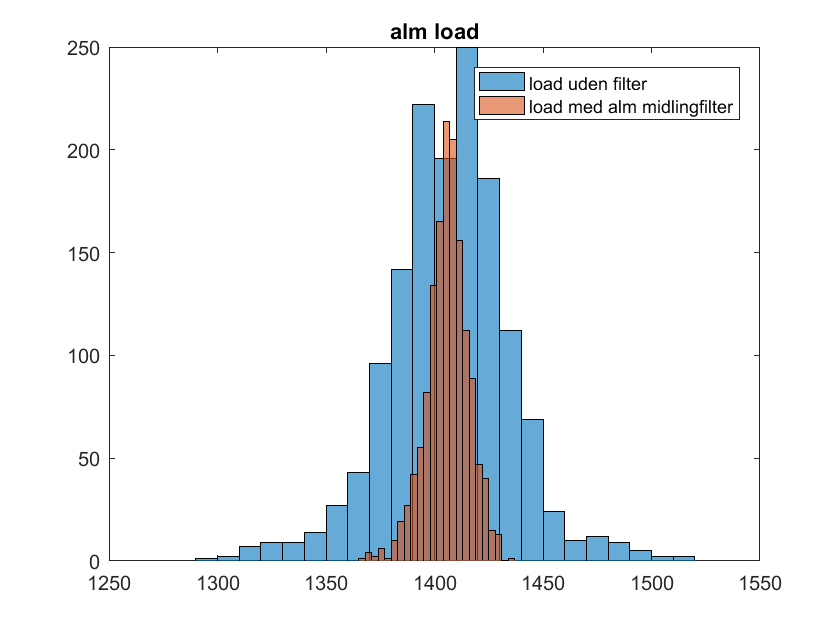
\includegraphics[width=90mm]{Img/Histogram_load_L.png}
	\caption{Histogram af load med og uden filter. Filterorden = 10}
	% \floatfoot{Source: (Citation command)}
	\label{fig:histogram1}
\end{figure}

Man kan se at filteret får vores data til at ligge tættere på hinanden, hvilket er det vi gerne vil se. Det samme kan ses for noload på \ref{fig:histogram2}

\begin{figure}[H]
	\centering
	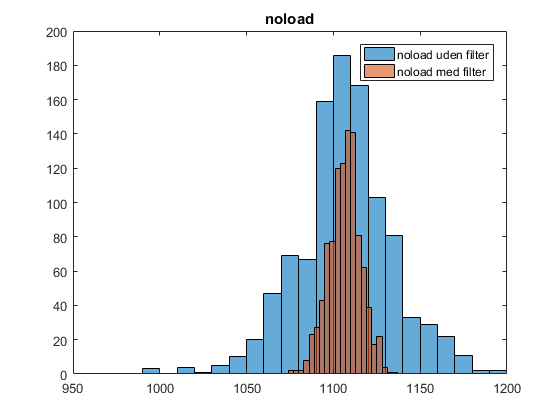
\includegraphics[width=90mm]{Img/Histogram_noload_L.png}
	\caption{Histogram af noload med og uden filter. Filterorden = 10}
	% \floatfoot{Source: (Citation command)}
	\label{fig:histogram2}
\end{figure}

Ved at ændre på ordnen kan man få filtret til at midle kraftigere. Dette kan ses på figur \ref{fig:histogram3}

\begin{figure}[H]
	\centering
	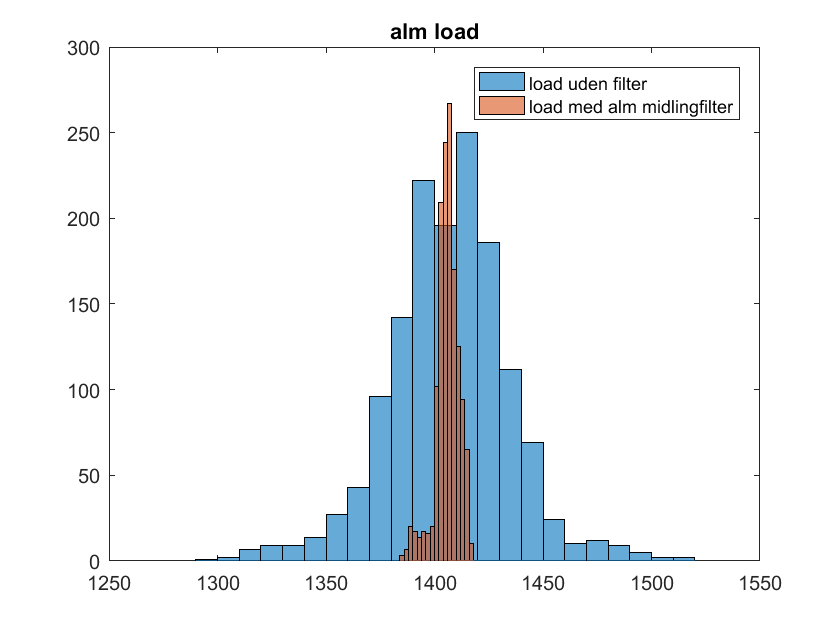
\includegraphics[width=90mm]{Img/Histogram_load_50.png}
	\caption{Histogram af load med og uden filter. Filterorden = 50}
	% \floatfoot{Source: (Citation command)}
	\label{fig:histogram3}
\end{figure}

Det ses tydligt at de orange pinde er blevet smallere og fylder et mindre område på grafen.\\
Hvis man kigger på varians og spredning kan man se at de stemmer godt overens med vores grafer. \\
\newpage

\begin{lstlisting}[frame=single]  % Start your code-block
for i:=maxint to 0 do

var_load = var(y_load)
var_noload = var(y_noload)

P_load = (1/sqrt(M)*S_load)^2
P_noload = (1/sqrt(M)*S_noload)^2
\end{lstlisting}

Ved M = 10 får vi en varians på ca 90, mod en varians på ca 25 ved en orden på 50. Hvis man kigger på støj-effekten ser man det samme. Ved en orden på 10 er støj-effekten ca 10 højere end ved en orden på 50.\\

Hvis man ønsker en max svingningstid for sit system, bliver man muligvis nødt til at begrænse sin orden på filteret. Hvis vi har et krav om en indsvingningstid på 100ms kan vi lave en hurtigt udregning:

\begin{lstlisting}[frame=single]  % Start your code-block
for i:=maxint to 0 do
maxKoef = fs*0.1;
\end{lstlisting}

Dette giver os et filter med en orden på 30. 
\subsection{Eksponentielt midlingsfilter}


\section{Opgave 3}

\section{Matlab kode}	

\end{document}